\documentclass[10pt]{article}
\usepackage[utf8]{inputenc}
\usepackage[T1]{fontenc}
\usepackage{amsmath}
\usepackage{amsfonts}
\usepackage{amssymb}
\usepackage[version=4]{mhchem}
\usepackage{stmaryrd}
\usepackage{soul}
\usepackage{graphicx}


\title{MATH1021}
\author{Mingyuan Ba}
\date{\today} % 

\begin{document}
\maketitle


\section{W1}
\begin{enumerate}

\item Terminology (Numbers and intervals). A number $r \in \mathbb{R}$ is called rational if there are integers $p, q \in \mathbb{Z}$ with $q \neq 0$ such that $r=p / q$. If it is not rational, it is called irrational. Interval notation if $a \leq b$ :

\begin{itemize}
  \item $(a, b):=\{x \in \mathbb{R} \mid a<x<b\}$ open interval

  \item $[a, b]:=\{x \in \mathbb{R} \mid a \leq x \leq b\}$ closed interval

  \item $[a, b):=\{x \in \mathbb{R} \mid a \leq x<b\}$ half open (or half closed) interval

  \item $(a, \infty):=\{x \in \mathbb{R} \mid a<x\}$ open half line

  \item $(-\infty, a]:=\{x \in \mathbb{R} \mid x \leq a\}$ closed half line

\end{itemize}

\item Terminology (Complex numbers). Complex numbers are numbers of the form $z=x+i y$ with $x$ and $y$ real numbers and imaginary unit $i$ having the property that $i^{2}=-1$. Any complex number represents a point on the plane with coordinates $(x, y)$. With that identification we obtain the complex plane or Argand diagram. We call $x+i y$ the Cartesian form of $z$. We have

\begin{itemize}
  \item \hl{$\operatorname{Re} z:=x$ is called the real part of $z$}

  \item \hl{$\operatorname{Im} z:=y$ is called the imaginary part of $z$}

  \item \hl{$\bar{z}:=x-i y$ is called the complex conjugate of $z=x+i y$}

  \item \hl{$|z|:=\sqrt{x^{2}+y^{2}}=\sqrt{z \bar{z}}$ is calle the modulus of $z$ (distance of $z$ from origin)}

  \item $\frac{z}{w}=\frac{z \bar{w}}{|w|^{2}}$ to make the denominator real

\end{itemize}

\item Computations work exactly the same as for real numbers, taking into account that $i^{2}=-1$.

Terminology (Sets). If $A, B$ are subsets of a larger set $X$ we define

\begin{itemize}
  \item the union of $A$ and $B: \quad A \cup B:=\{x \in X \mid x \in A$ or $x \in B\}$;

  \item the intersection of $A$ and $B: A \cap B:=\{x \in X \mid x \in A$ and $x \in B\}$;

  \item the complement of $A: \quad A^{c}:=\{x \in X \mid x \notin A\}$;

  \item the complement of $B$ in $A: A \backslash B:=A \cap B^{c}=\{x \in A \mid x \notin B\}$.

\end{itemize}

\end{enumerate}

\newpage



\section{W2}

\begin{enumerate}
\item Definition (Polar form, complex exponential function). A complex number $z$ with modulus $|z|=r$ and $\operatorname{argument} \arg (z)=\theta$ can be written in \hl{standard polar form} as

$$
z=r(\cos (\theta)+i \sin (\theta))
$$

or shorter in \hl{exponential polar form}

$$
z=r e^{i \theta}
$$

where by definition $e^{i \theta}:=\cos (\theta)+i \sin (\theta)$ for all $\theta \in \mathbb{R}$ \hl{measured in radians}. Note that $\theta \mapsto e^{i \theta}$ is $2 \pi$-periodic, that is, \hl{$e^{i(\theta+2 \pi k)}=e^{i \theta}$} for all $k \in \mathbb{Z}$. More generally we define the complex exponential function

$$
e^{z}=e^{x+i y}=e^{x} e^{i y}=e^{x}(\cos y+i \sin y) .
$$

for all $z=x+i y$ with $x, y \in \mathbb{R}$.
\\\\
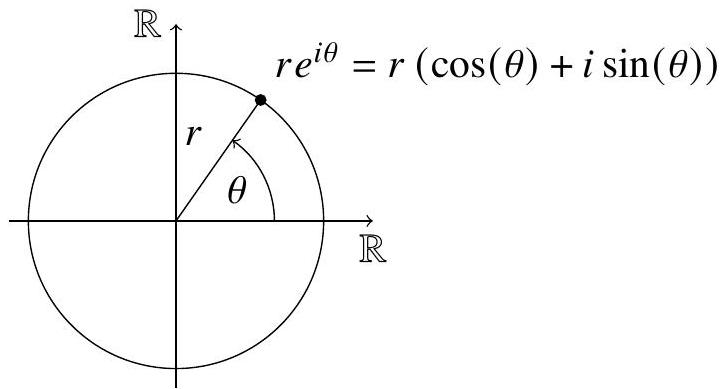
\includegraphics[width=0.8\textwidth]{images/W2-1.jpg}


Note : The complex exponential function has the same properties as the usual exponential function. For $z, w \in \mathbb{C}$ we have\\


$$
e^{0}=1, \quad e^{z} e^{w}=e^{z+w}, \quad e^{-z}=\frac{1}{e^{z}} .
$$

\textit{W2-Exercises-Q8}


\newpage

\item \hl{Theorem (De Moivre's Theorem). For any $n \in \mathbb{Z}$,}


$$
(\cos (\theta)+i \sin (\theta))^{n}=\cos (n \theta)+i \sin (n \theta) .
$$



or in exponential polar form (more intuitive and natural)

$$
\left(e^{i \theta}\right)^{n}=e^{i n \theta}
$$

corresponding to the usual index laws for powers.

\textit{W2-Exercises-Q7(f)}
\textit{W2-Exercises-Q9}
\textit{W2-Exercises-Q10}
\textit{W2-TUT-Q4}


\item Additional typical problem
\textit{W2-Exercises-Q12}
\textit{W2-Exercises-Q13}
\textit{W2-Exercises-Q14}
\textit{W2-TUT-Q6}
\textit{W2-TUT-Q7}
\end{enumerate}


\newpage


\section{W3}

\begin{enumerate}
\item Terminology (Functions). Let $A, B \subseteq \mathbb{R}$ be sets. A function $f: A \rightarrow B$ is a rule which assigns exactly one element of $B$ to each element of $A$. We call \hl{$A$ the domain} of $f$ and\hl{ $B$ the codomain} of $f$. The graph of $f$ is the set $\{(x, f(x)) \mid x \in A\}$. \hl{For a function we require that every vertical line through $x \in A$ meets the graph at exactly one point.}

\item If $f(x)$ is given by a formula, the \hl{natural domain} is the set of $x \in \mathbb{R}$ such that the formula makes sense, for instance $\log (x)$ makes sense for $x>0$, so $A=(0, \infty)$ is the natural domain.\\\\
\textit{W3-Exercises-Q2}
\textit{W3-Exercises-Q6}
\textit{W3-TUT-Q3}

\item The \hl{range} of $f$ is the set $\{f(x) \mid x \in A\}$. \hl{We call the function $f$ is surjective or onto if the range is $B$(\textit{Range = Codomain}). For $f$ to be surjective, every horizontal line through $y \in B$ meets the graph at least once.}\\
\textit{W3-Exercises-Q7}
\textit{W3-Exercises-Q8}

\item \hl{The function $f$ is injective or one-to-one if every point in the image comes from exactly one element in the domain. For $f$ to by injective every horizontal line through $y \in B$ meets the graph at most once, that is, exactly once or not at all.}\\
\textit{W3-Exercises-Q10}

\item The function $f$ is \hl{bijective or invertible}if it is both injective and surjective. \hl{Then the equation $y=f(x)$ has a unique solution $x \in A$ for each $y \in B$. }The inverse function $f^{-1}: B \rightarrow A$ recovers the value of $x \in A$ from the value of $y \in B$. To find $f^{-1}$, solve $y=f(x)$ for $x \in A$, then swap the names of the variables. \hl{The graph of $f^{-1}: B \rightarrow A$ is obtained by reflecting the graph of $f$ at the diagonal $x=y$.}\\\\
\textit{W3-Exercises-Q1}
\textit{W3-Exercises-Q11}
\textit{W3-TUT-Q2}
\textit{W3-TUT-Q6}
\textit{W3-TUT-Q7}

\newpage


\item Definition (hyperbolic sine and cosine functions.). The hyperbolic cosine and hyperbolic sine functions are defined by

$$
\begin{aligned}
& \cosh (x):=\frac{e^{x}+e^{-x}}{2} \\
& \sinh (x):=\frac{e^{x}-e^{-x}}{2}
\end{aligned}
$$

for all $x \in \mathbb{R}$. They share many properties with the cosine and sine functions.


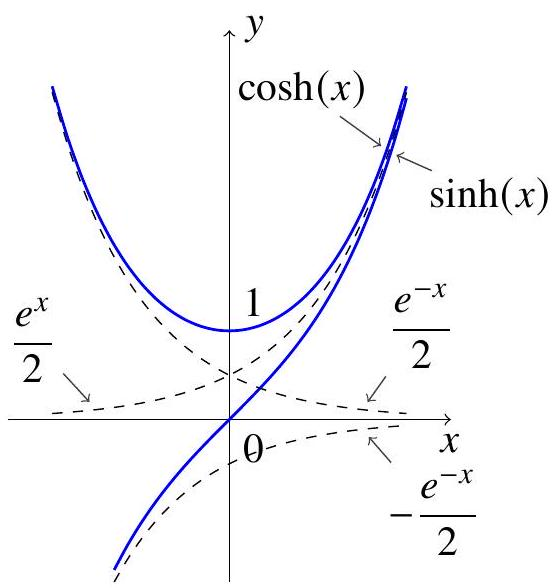
\includegraphics[width=0.6\textwidth]{images/W3-1.jpg}\\
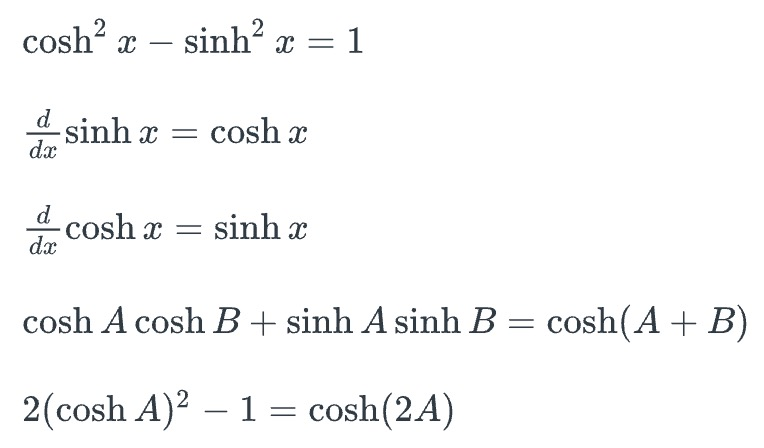
\includegraphics[width=0.8\textwidth]{images/W3-3.jpg}\\
\textit{W3-TUT-Q5}

\newpage

\item Composite function\\
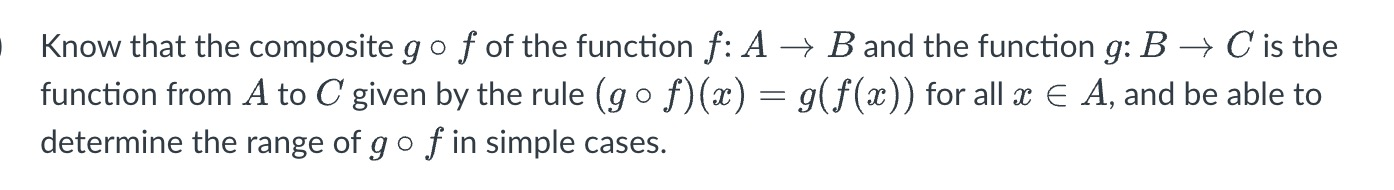
\includegraphics[width=1\textwidth]{images/W3-2.jpg}\\
\textit{W3-Exercises-Q6}
\textit{W3-TUT-Q4}



\item Additional typical problem:\\\\
\textit{W3-Exercises-Q5}

\end{enumerate}


\newpage



\section{W4}
\begin{enumerate}
\item One side limit:\\\\
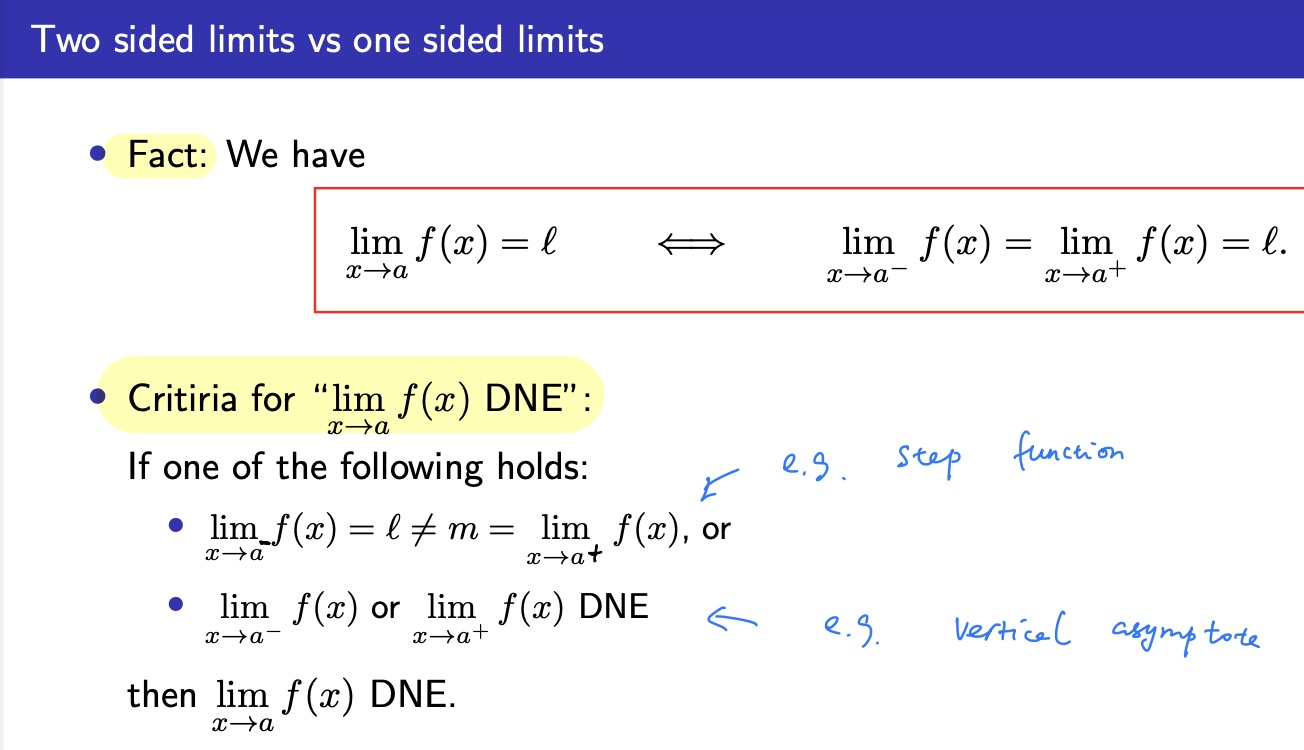
\includegraphics[width=0.9\textwidth]{images/W4-2.jpg}\\

\item DNE problem:\\\\
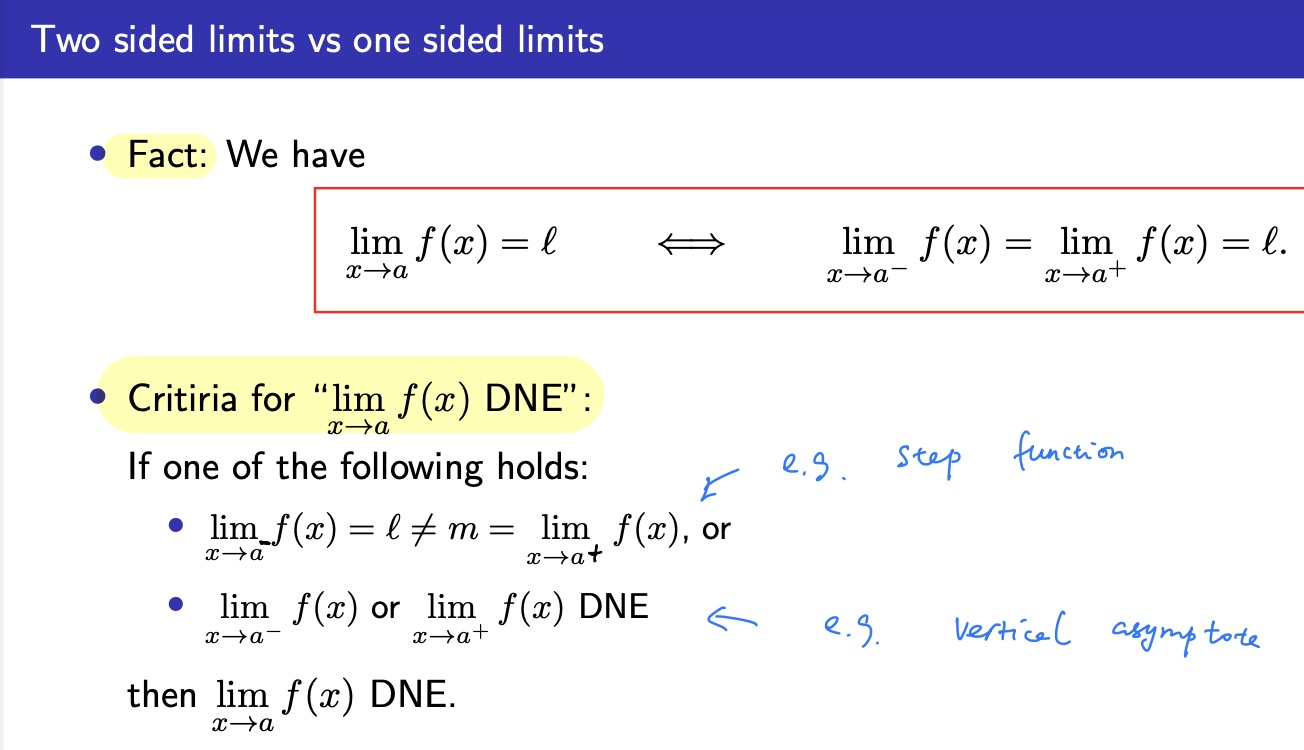
\includegraphics[width=1\textwidth]{images/W4-2.jpg}\\

\item \textit{Note}:\\Limits are usually computed by using some \hl{elementary limits and the limit and squeeze laws.}

\newpage

\item Limit Laws. If $\lim _{x \rightarrow a} f(x)=\ell$ and $\lim _{x \rightarrow a} g(x)=m$, then

\begin{itemize}
  \item $\lim _{x \rightarrow a}(k f(x))=k \ell$ for all $k \in \mathbb{R}$.

  \item $\lim _{x \rightarrow a}(f(x) g(x))=\ell m$

  \item $\lim _{x \rightarrow a}(f(x)+g(x))=\ell+m$

  \item $\lim _{x \rightarrow a} \frac{f(x)}{g(x)}=\frac{\ell}{m}$ provided $m \neq 0$

\end{itemize}

\item \hl{Squeeze Law. Suppose that $f(x) \leq g(x) \leq h(x)$ for all $x \neq a$ near $a$. If $\lim _{x \rightarrow a} f(x)=\ell$ and $\lim _{x \rightarrow a} h(x)=\ell$, then $\lim _{x \rightarrow a} g(x)=\ell$.}\\
\textit{W4-Exercises-Q5}
\textit{W4-TUT-Q4}

\item Elementary limits:\\Frequently used elementary limits are $\lim _{x \rightarrow 0} \frac{\sin (x)}{x}=1$. Roots $\lim _{x \rightarrow a} \sqrt[n]{x}=\sqrt[n]{a}$ $(a>0)$ and other elementary functions allow the computation of limits by substitution (they are continuous, see below).\\
\textit{W4-Exercises-Q7}

\item Limits with fractions:\\Limits of the form $\lim _{x \rightarrow \infty} \frac{f(x)}{g(x)}$ are often computed \hl{by dividing numerator and denomintor by the fastest growing term, often the highest power of $x$.}\\
\textit{W4-Exercises-Q3}
\textit{W4-Exercises-Q4}
\textit{W4-TUT-Q2}
\textit{W4-TUT-Q3}

\newpage

\item Definition of continutity:\\A function $f$ is \hl{continuous} at a point $a$ if $a$ is in the domain of $f$ and $\lim _{x \rightarrow a} f(x)=f(a)$, that is, the limit exists and equals the function value at $a$. We often make use of the fact that elementary functions such as polynomials, roots, exponentials and the trigonometric functions are continuous.

\begin{itemize}
\item \textbf{continuity at a point}\\
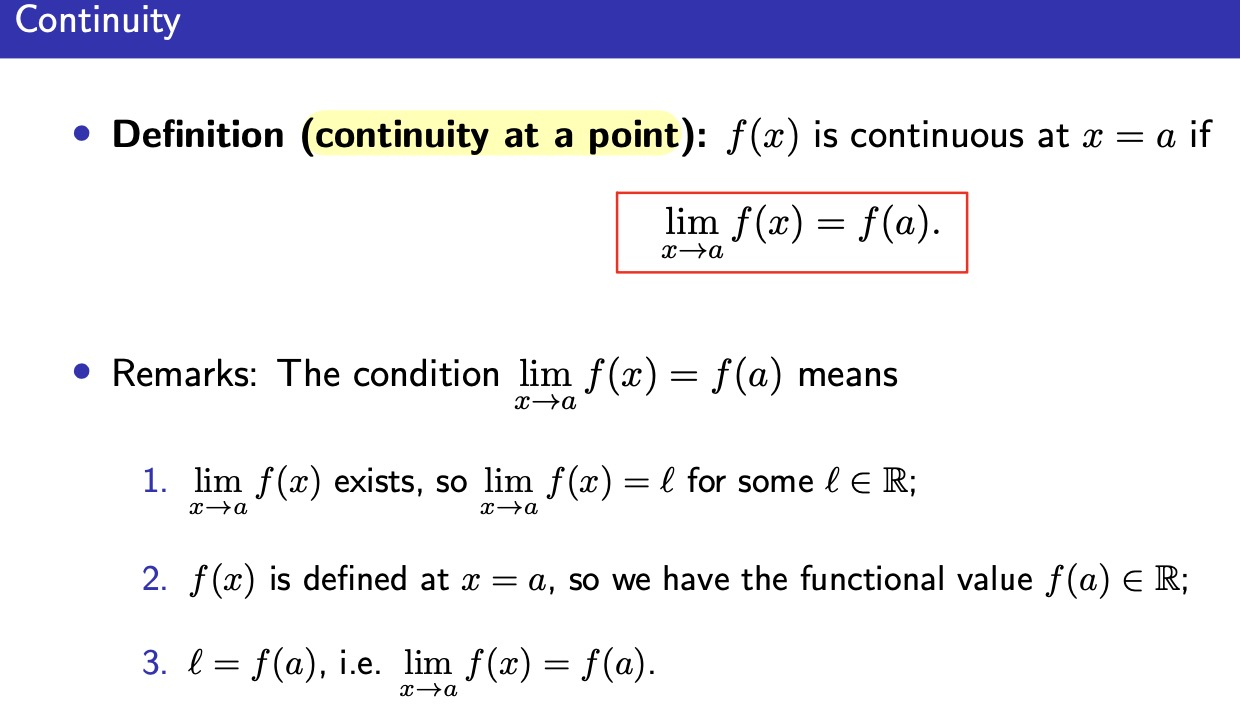
\includegraphics[width=1\textwidth]{images/W4-3.jpg}\\

\item \textbf{Variations of the theme of continuity}\\
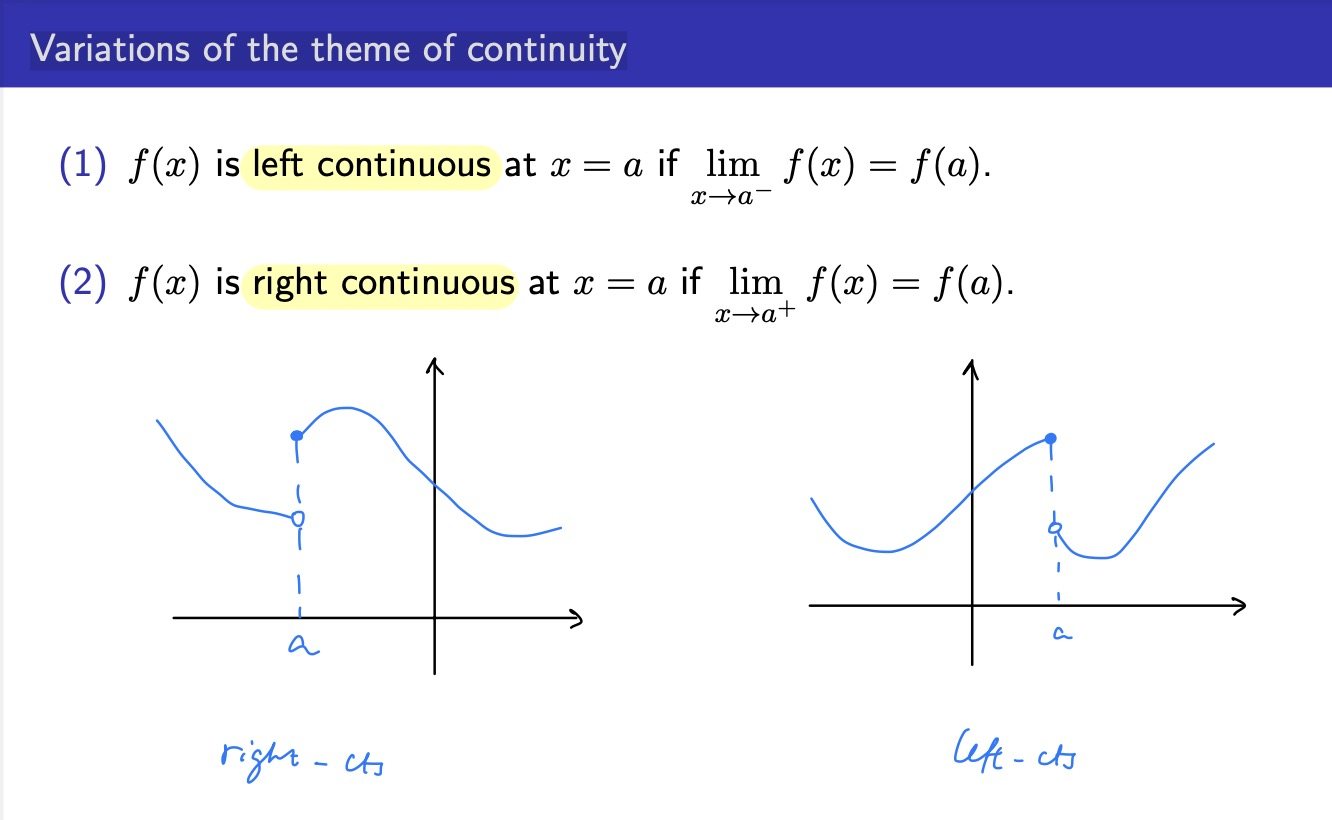
\includegraphics[width=1\textwidth]{images/W4-4.jpg}\\
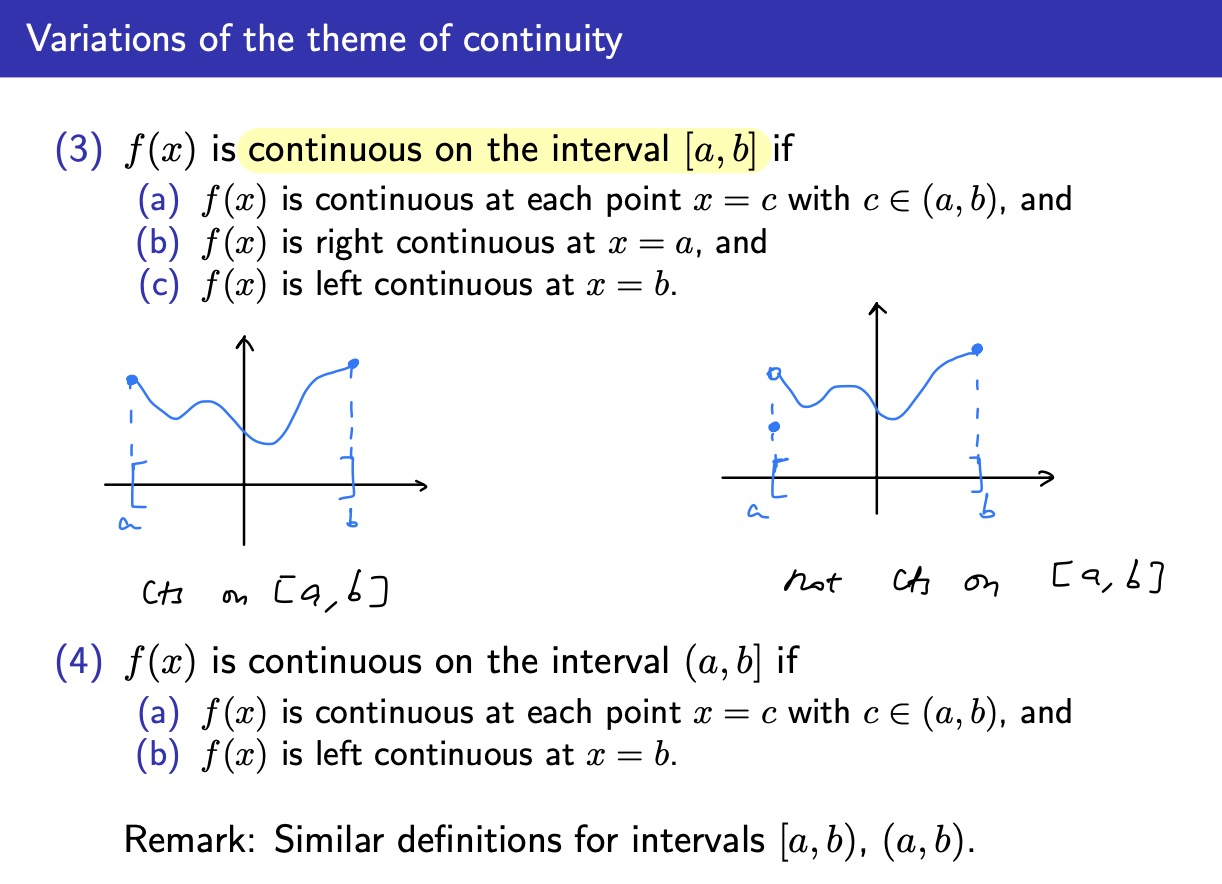
\includegraphics[width=1\textwidth]{images/W4-5.jpg}\\

\item \textbf{Limits of continuous functions}\\
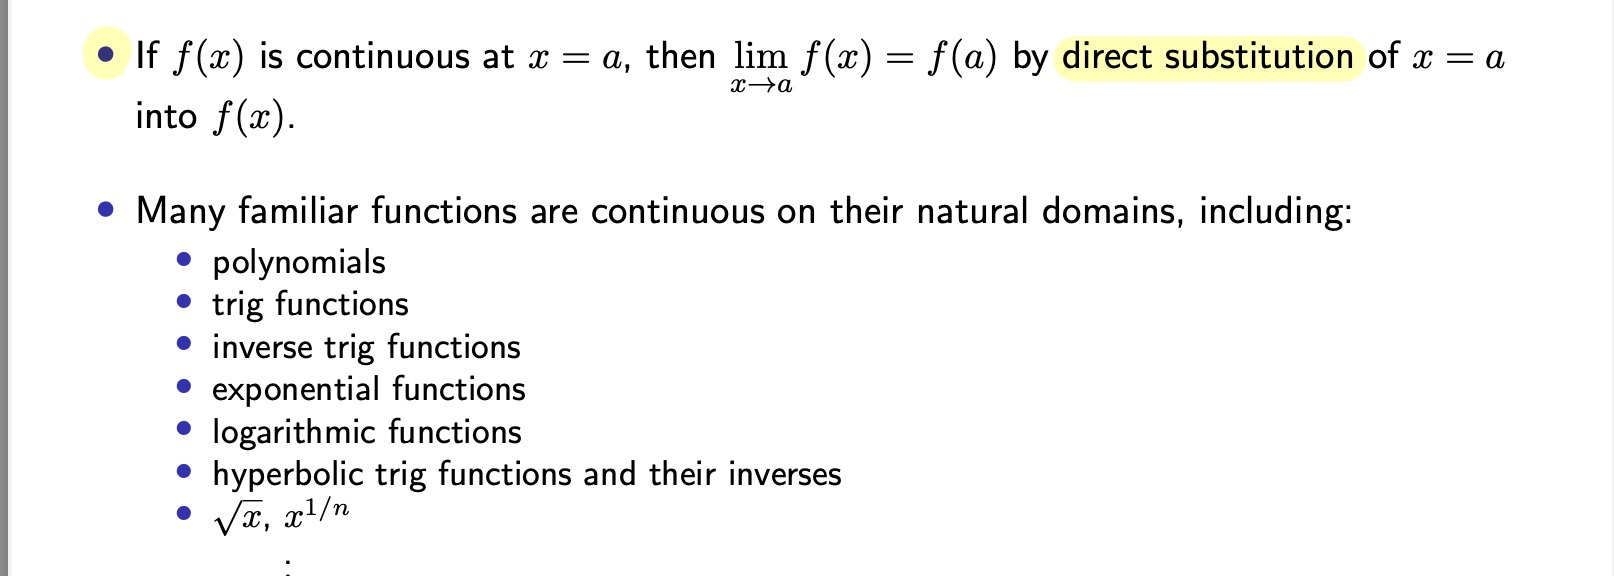
\includegraphics[width=1\textwidth]{images/W4-6.jpg}\\\\
\textit{W4-TUT-Q6}
\textit{W4-TUT-Q7}
\textit{W4-TUT-Q8}

\item \textbf{Composition Law}\\
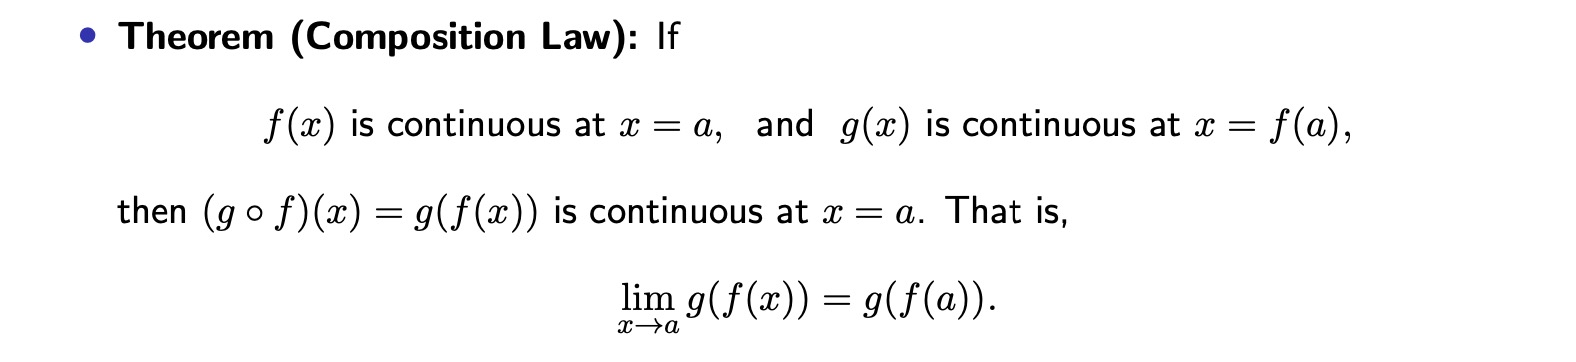
\includegraphics[width=1\textwidth]{images/W4-7.jpg}\\

\end{itemize}



\end{enumerate}


\newpage



\section{W5}

\begin{enumerate}

\item \textbf{Definition (Derivative):}\\
The derivative of a function $f$ at $x_{0}$ is the \hl{slope of the tangent to the graph of $f$ at the point $\left(x_{0}, f\left(x_{0}\right)\right)$.} If it exists, it is the limit of the difference quotient

$$
f^{\prime}\left(x_{0}\right):=\lim _{x \rightarrow x_{0}} \frac{f(x)-f\left(x_{0}\right)}{x-x_{0}}=\lim _{h \rightarrow 0} \frac{f\left(x_{0}+h\right)-f\left(x_{0}\right)}{h} .
$$

Derivatives also represent rates of change.

\item \textbf{Note (Rules of Differentiation):} \\
If $f(x)$ and $g(x)$ are differentiable, then the following functions are also differentiable, with derivatives as stated:\\
(1) $(\alpha f)^{\prime}=\alpha f^{\prime}$ for $\alpha \in \mathbb{R}$\\
(2) $\left(\frac{f}{g}\right)^{\prime}=\frac{f^{\prime} g-f g^{\prime}}{g^{2}}$ (if $g^{\prime}(x) \neq 0$, quotient rule)\\
(3) $(f+g)^{\prime}(x)=f^{\prime}+g^{\prime}$\\
(4) $(f g)^{\prime}=f^{\prime} g+f g^{\prime}($ product rule)\\
(5) \hl{$(f \circ g)^{\prime}(x)=g^{\prime}(x) f^{\prime}(g(x))$ (chain rule)}\\

\item \textbf{Note (Implicit differentiation):}\\
\hl{Functions can be given implicitly by an equation such as $f(x, y)=c$, where $c$ is a constant. For example $\cos (y)+x y=3$. Assuming that $y$ is a function of $x$ we use the rules of differentiation to take the derivative. Since the derivative of a constant is zero differentiation with respect to $x$ is given by $\sin (y) y^{\prime}+x=0$. Solve for $y^{\prime}$ to get the derivative.}

\end{enumerate}


\newpage

\section{W6}

\begin{enumerate}
\item \textbf{Note:}\\
Suppose that $f:[a, b] \rightarrow \mathbb{R}$ is differentiable with a continuous derivative.

\begin{itemize}
  \item If $f^{\prime}(x)>0[<0]$ on some interval $(c, d)$, then $f$ is strictly increasing [decreasing] on $(c, d)$.

  \item If $f^{\prime \prime}(x)>0[<0]$ on some interval $(c, d)$, then $f$ is concave up [down] on $(c, d)$.

  \item If $f$ has a (local) maximum or minimum at some $c \in(a, b)$, then $f^{\prime}(c)=0$.

  \item If $f^{\prime}(c)=0$ and $f^{\prime \prime}(c)<0$, then $f$ has a local maximum at $x=c$. Likewise, if $f^{\prime}(c)=0$ and $f^{\prime \prime}(c)>0$, then $f$ has a minimum at $x=c$. (In both cases $f^{\prime \prime}$ needs to be continuous)

  \item If $f$ has a point of inflection at $x=c$, then $f^{\prime \prime}(c)=0$.

  \item If $f^{\prime \prime}(c)=0$ and the sign of $f^{\prime \prime}$ changes at $x=c$, then $f$ has a point of inflection at $x=c$.

  \item The function $f$ has a global maximum [minimum] at some $c \in[a, b]$ with $f^{\prime}(c)=0$ if $c \in(a, b)$.

\end{itemize}

\item \textbf{Method (L'Hôpital's rule):}\\
\hl{L'Hôpital's rule is a method to compute limits of fractions that lead to indeterminate expressions of the form $0 / 0$ or $\pm \infty / \pm \infty$. If $f, g$ are such that $f(x) \rightarrow 0$ and $g(x) \rightarrow 0$ as $x \rightarrow a$ and}

$$
\lim _{x \rightarrow a} \frac{f^{\prime}(x)}{g^{\prime}(x)}=L
$$

exists, then

$$
\lim _{x \rightarrow a} \frac{f(x)}{g(x)}=L
$$

A similar statement holds if $f(x) \rightarrow \infty$ and $g(x) \rightarrow \infty$ as $x \rightarrow a$. It is also valid if $a= \pm \infty$ or $L \pm \infty$.

\end{enumerate}

\newpage


\section{W7}

\begin{enumerate}

\item \textbf{Note (Taylor polynomial):}\\
The $n$-th order Taylor polynomial $T_{n}$ of a $n$ times differentiable function $f$ at a point $a$ is the polynomial of degree at most $n$ providing the best possible approximation of $f$ near a. It is given by

$$
\begin{aligned}
T_{n}(x)=f(a) & +f^{\prime}(a)(x-a)+\frac{f^{\prime \prime}(a)}{2}(x-a)^{2} \\
& +\cdots+\frac{f^{(k)}(a)}{k !}(x-a)^{k}+\cdots+\frac{f^{(n)}(a)}{n !}(x-a)^{n}
\end{aligned}
$$

\textbf{Note} that $f^{(k)}(a)=T_{n}^{(k)}(a)$ for $k=0, \ldots, n$. We call $T_{n}$ the $n$-th order Taylor polynomial of $f$ about $x=a$.


\textbf{Substitution method:}\\
If $T_{n}$ is the $n$-th order Taylor polynomial of $f$ about $a=0$ and $m \in \mathbb{N}$, then $T_{n}\left(x^{m}\right)$ is the Taylor polynomial of order $m n$ of $f\left(x^{m}\right)$ about 0 .

\item \textbf{Note (Lagrange form of remainder):}\\
\hl{If $T_{n}$ is the $n$-th order Taylor polynomial of $f$ centred at $a$ we call}

$$
R_{n}(x)=f(x)-T_{n}(x)
$$

\hl{the $n$-th order remainder. It satsifies the limit}

$$
\lim _{x \rightarrow a} \frac{R_{n}(x)}{(x-a)^{n}}=0
$$

\hl{If $f$ has $n+1$ derivatives, then $R_{n}(x)$ can be represented in the Lagrange form: There exists $c$ strictly between $a$ and $x$ such that}

$$
R_{n}(x)=\frac{f^{(n+1)}(c)}{(n+1) !}(x-a)^{n+1}
$$

It is almost like the $(n+1)$-st term, but with $f^{(n+1)}(a)$ replaced by $f^{(n+1)}(c)$.

\end{enumerate}


\newpage



\section{W8}
\begin{enumerate}

\item \textbf{Note (Taylor series expansion):}\\
The Taylor series expansion of a function $f$ at a point $a$ is the limit of Taylor the polynomials. It represents the function $f$ if

$$
f(x)=\sum_{k=0}^{\infty} \frac{f^{(k)}(a)}{n !}(x-a)^{k}=\lim _{n \rightarrow \infty} \sum_{k=0}^{n} \frac{f^{(k)}(a)}{n !}(x-a)^{k} .
$$

If $T_{n}(x)$ is the $n$-th order polynomial and $R_{n}(x)=f(x)-T_{n}(x)$, then the Taylor series represents $f$ if $R_{n}(x) \rightarrow 0$ as $n \rightarrow \infty$. \hl{To show this we use the Lagrange form of remainder given by}

$$
R_{n}(x)=\frac{f^{(n+1)}(c)}{(n+1) !}(x-a)^{n+1}
$$

for some $c$ between $x$ and $a$. Often, $\left|R_{n}(x)\right|$ is maximised over $c$ between $a$ and $x$ to show that $\left|R_{n}(x)\right| \rightarrow 0$.

\item \textbf{Note (Geometric series):}\hl{If $x \neq 1$, then for every $n \in \mathbb{N}$ we have}

$$
1+x+x^{2}+\cdots+x^{n}=\frac{1-x^{n+1}}{1-x}
$$

and if $|x|<1$, then

$$
\frac{1}{1-x}=\lim _{n \rightarrow \infty} \frac{1-x^{n+1}}{1-x}=\sum_{k=0}^{\infty} x^{k}
$$

\end{enumerate}


\newpage




\section{W9}
\begin{enumerate}

\item Definition (Riemann sums). Let $f$ be a continuous function on an interval $[a, b]$ and let $a=x_{0}<x_{1}<$ $x_{2}<\cdots<x_{N}=b$ be a partition (subdivision) of $[a, b]$ into $N$ intervals $\left[x_{k-1}, x_{k}\right]$ of equal length (for simplicity). Then

$$
\Delta x=\frac{b-a}{N}
$$

is the length of these intervals and $x_{k}=a+k \Delta x$ for $k=0, \ldots, N$. Choose points a point $x_{k}^{*}$ from each of the intervals $\left[x_{k-1}, x_{k}\right]$. The sum

$$
\sum_{k=1}^{N} f\left(x_{k}^{*}\right) \Delta x
$$

is called a Riemann sum. It approximates the area of the region under the graph $y=f(x)$ given by sums of the area of rectangles as shown below.

\begin{center}
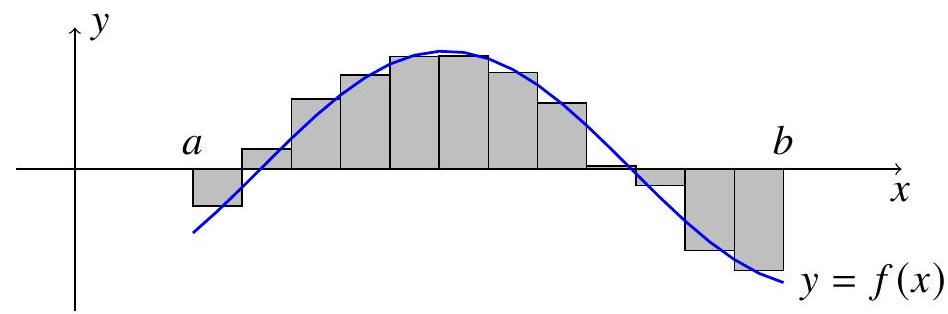
\includegraphics[width=0.8\textwidth]{images/W9-1.jpg}\\
\end{center}

\item The limit of these sums as $N \rightarrow \infty$ is the definite integral of $f$ over $[a, b]$, denoted by

$$
\lim _{N \rightarrow \infty} \sum_{k=1}^{N} f\left(x_{k}^{*}\right) \Delta x=\int_{a}^{b} f(x) d x .
$$

\item \textbf{Note (Upper and lower Riemann sums):}\\
If we choose $x_{k}^{*}$ such that $f\left(x_{k}^{*}\right)$ is the maximum (or minimum) of $f$ on $\left[x_{k-1}, x_{k}\right]$, then the corresponding Riemann sum is called the upper (or lower) Riemann sum. We denote them by $U_{N}$ and $L_{N}$, respectively. We have

$$
L_{N} \leq \int_{a}^{b} f(x) d x \leq U_{N}
$$

If the function is \hl{increasing, then for $x^{*} k$ choose the left endpoint of $\left[x_{k-1}, x_{k}\right]$ for the lower sum and the right endpoint for the upper sum. }For a decreasing function it is the other way.

\end{enumerate}


\newpage



\section{W10}

\begin{enumerate}

\item Theorem (Fundamental Theorem of Calculus.). The fundamental theorem of calculus makes a connection between integration and differentiation. It comes in two parts.

Part I If $f:[a, b] \rightarrow \mathbb{R}$ is continuous, then

$$
\frac{d}{d x} \int_{c}^{x} f(t) d t=f(x) \quad \text { for all } x \in[a, b]
$$

\textit{W10-Exercises-Q3}
\textit{W10-Exercises-Q4}
\textit{W10-TUT-Q3}
\textit{W10-TUT-Q4}
\textit{W10-TUT-Q5}


Part II If $F:[a, b] \rightarrow \mathbb{R}$ is differentiable and $F^{\prime}:[a, b] \rightarrow \mathbb{R}$ is continuous, then

$$
F(b)-F(a)=\int_{a}^{b} F^{\prime}(t) d t
$$

\item \textbf{Note:}\\
As a consequence of Part I we also have

$$
\frac{d}{d x} \int_{x}^{c} f(t) d t=-f(x) \quad \text { for all } x \in[a, b]
$$

and \hl{if $g$ is a differentiable function}, then the chain rule implies that

$$
\frac{d}{d x} \int_{c}^{g(x)} f(t) d t=f(g(x)) g^{\prime}(x) \quad \text { for all } x \in[a, b]
$$

and \hl{f $a$ and $b$ is a differentiable function}, then the chain rule implies that

$$
\frac{d}{d x} \int_{a(x)}^{b(x)} f(t) d t=f(b(x)) b^{\prime}(x) - f(a(x)) a^{\prime}(x)\quad \text { for all } x \in[a, b]
$$

\end{enumerate}


\newpage



\section{W11}
The following methods of integration are frequently used:
\begin{enumerate}

\item \hl{Change of variable formula (for definite integrals)\\}Integration by substitution \hl{Setting $s=u(t)$ we have $d s=u^{\prime}(s) d t$} and

$$
\int_{u(a)}^{u(b)} f(s) d s=\int_{a}^{b} f(u(t)) u^{\prime}(t) d t
$$

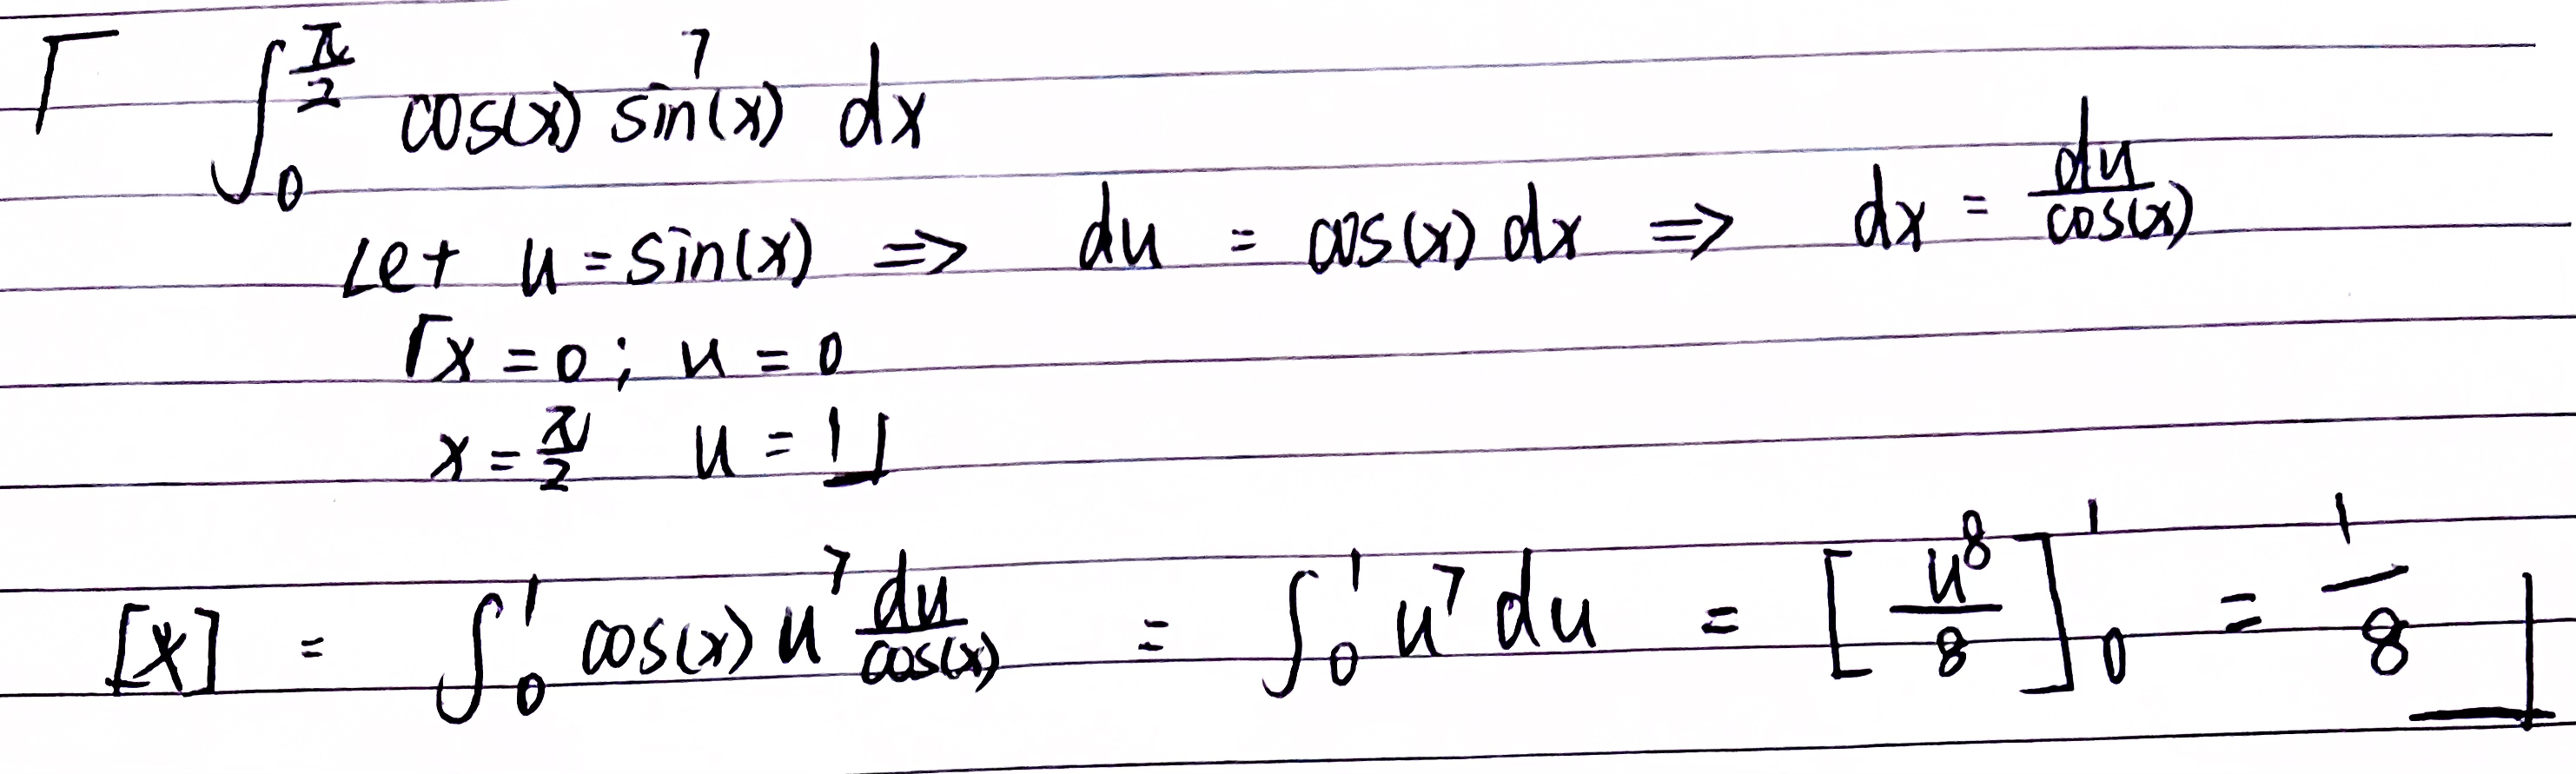
\includegraphics[width=0.8\textwidth]{images/W11-2.jpeg}


\hl{Change of variable formula (for indefinite integrals)}

\[
\int f(u(x)) u'(x)\, dx = \int f(u)\, du
\]

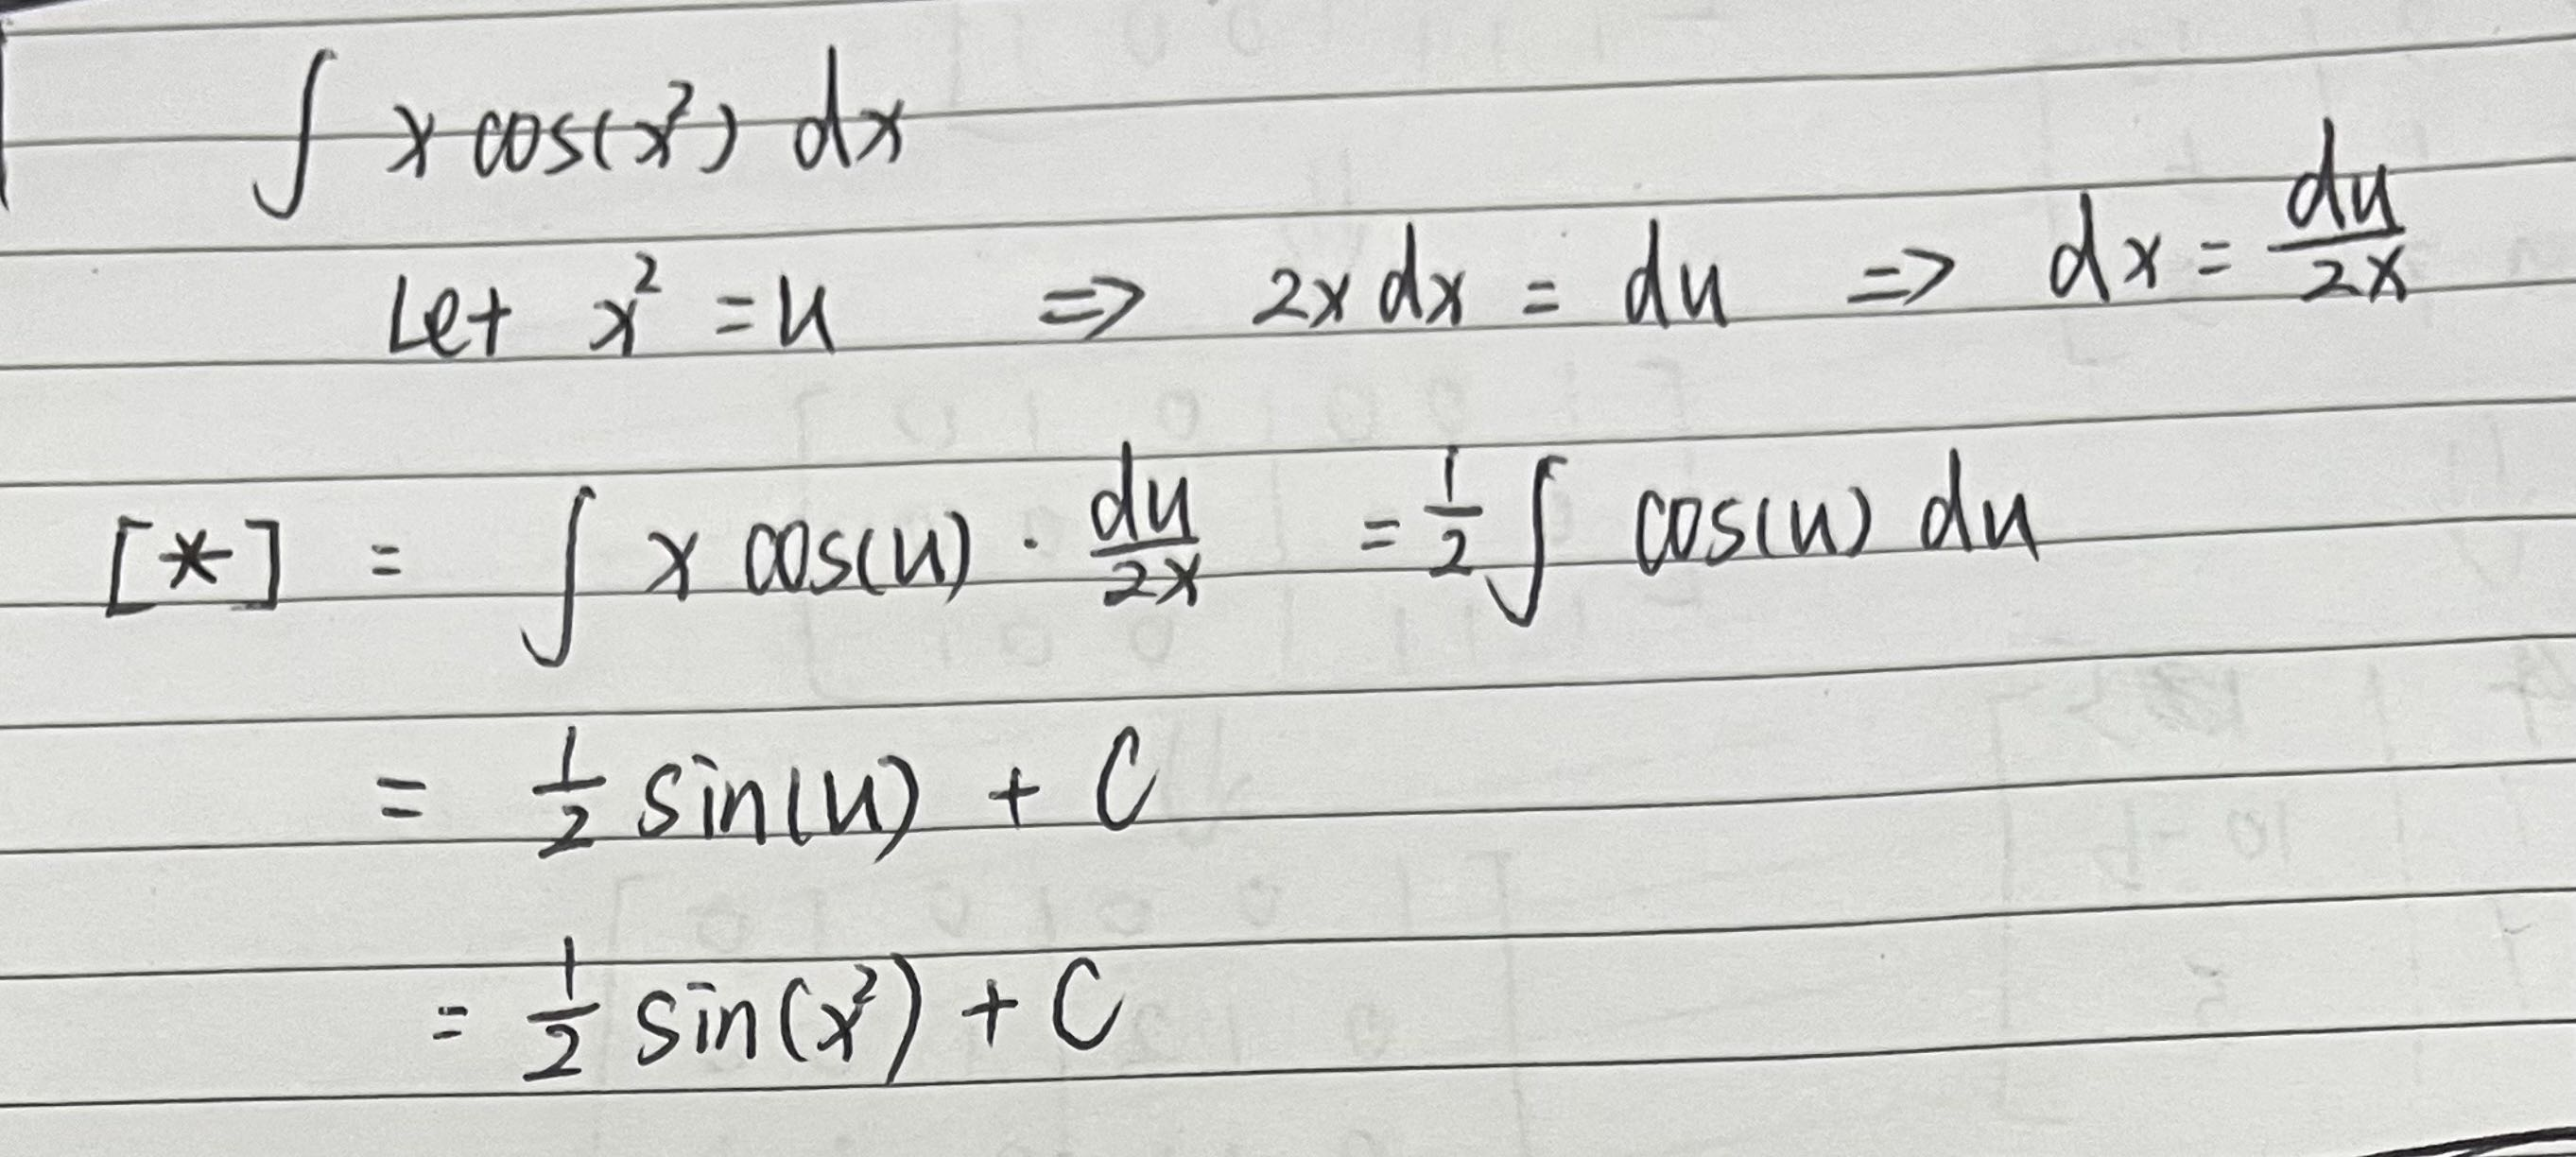
\includegraphics[width=0.8\textwidth]{images/W11-1.jpeg}\\


\newpage



\textbf{\textit{appendix:\\Trig substitution\\The trigonometric substitution method is a technique used in calculus to simplify integrals involving radicals. It involves substituting trigonometric functions for the variables in the integral. The most common trigonometric substitutions are:}}\\

\begin{itemize}
  \item For $\sqrt{a^2-x^2}$, where $a > 0$, we use the substitution $x = a\sin\theta$ ($-\frac{\pi}{2} \leq \theta \leq \frac{\pi}{2}$).
  
  \item For $\sqrt{a^2+x^2}$, we use the substitution $x = a\tan\theta$ ($-\frac{\pi}{2} < \theta < \frac{\pi}{2}$).
  
  \item For $\sqrt{x^2-a^2}$, where $a > 0$, we use the substitution $x = a\sec\theta$ ($0 \leq \theta < \frac{\pi}{2}$ or $\pi \leq \theta < \frac{3\pi}{2}$).
\end{itemize}


\textbf{\textit{These substitutions help in simplifying the integrals by expressing the radical term in terms of trigonometric functions, which often leads to easier calculations and solution of the integral.}}\\

Example:\\
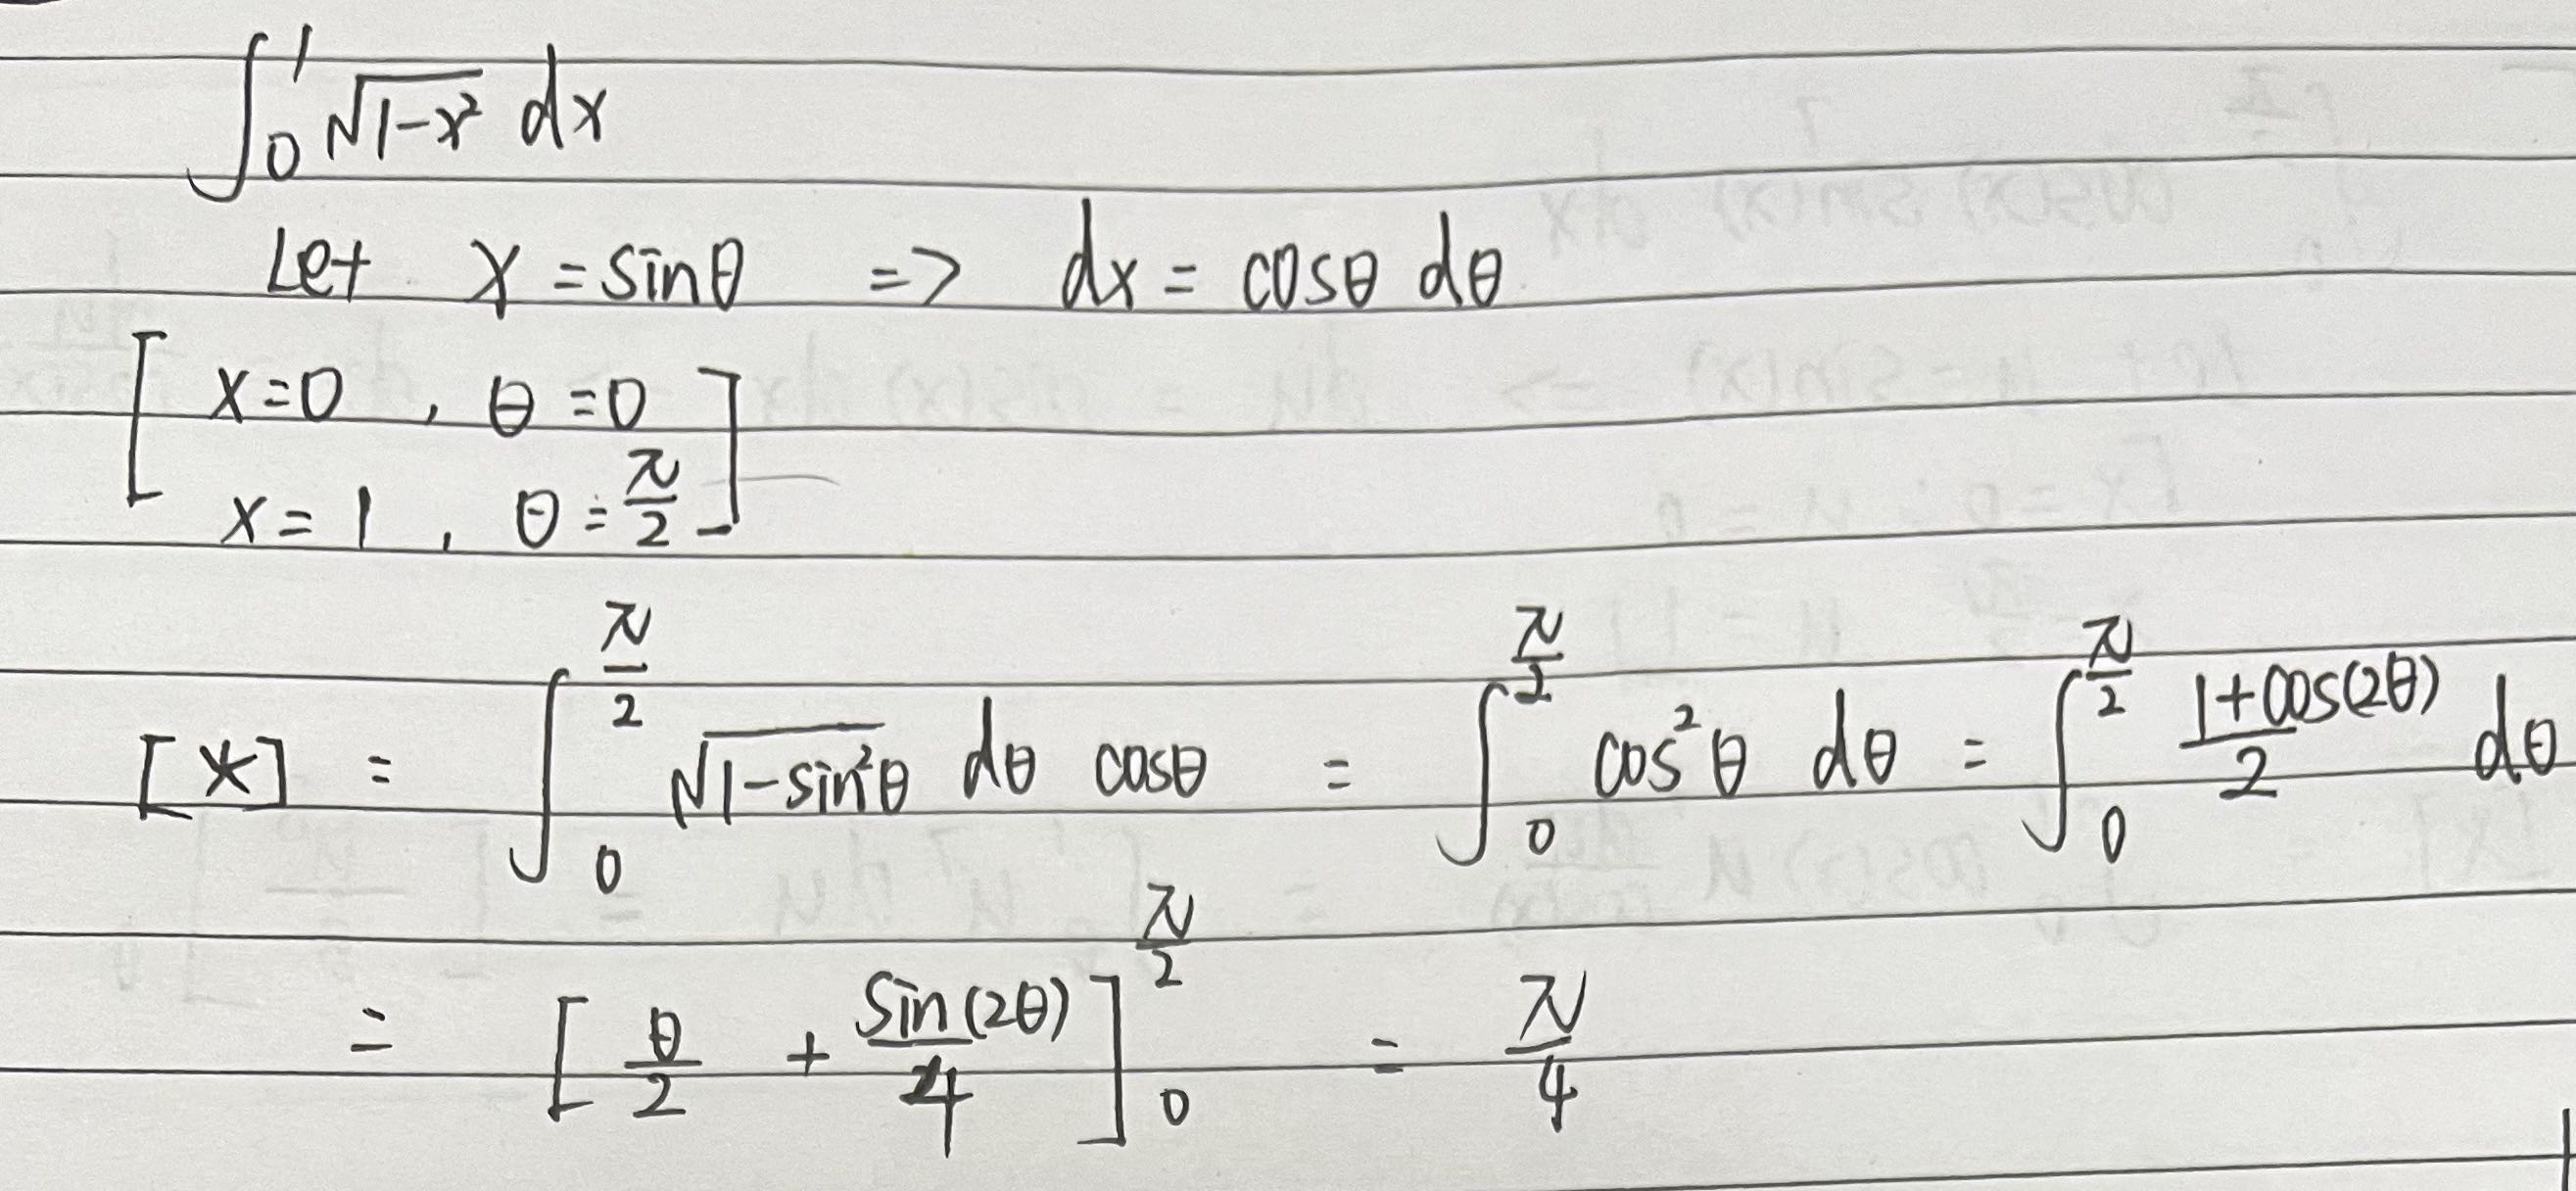
\includegraphics[width=0.8\textwidth]{images/W11-3.jpeg}\\

\item Integration by parts We have

$$
\int u \frac{d v}{d x} d x=u v-\int \frac{d u}{d x} v d x
$$

\item Integration by partial fractions Assume that $f$ can be written in the form

$$
f(x)=\frac{a+b x}{(x-\lambda)(x-\mu)}
$$

with $\lambda \neq \mu$ by possibly factorising the numerator. Write

$$
f(x)=\frac{A}{x-\lambda}+\frac{B}{x-\mu}=\frac{A(x-\mu)+B(x-\lambda)}{(x-\lambda)(x-\mu)}
$$

and determine $A, B$ by equating $A(x-\mu)+B(x-\lambda)=a x+b$. The easiest way is to choose $x=\lambda$ and $x=\mu$ to determine $A$ and $B$ in terms of $a, b, \mu, \lambda$.


\end{enumerate}





\section{W12}
\begin{enumerate}
\item \textbf{Note (Area between graphs):}\\
Let $f, g:[a, b] \rightarrow \mathbb{R}$ be continuous funcitons with $f(x) \geq g(x)$ for all $x \in[a, b]$. Then the region between the graphs has surface area given by

$$
\int_{a}^{b} f(x)-g(x) d x
$$

If the graphs cross over, one has to compute sum of the surface areas between the cross-over points to make sure it has the correct positive sign.

\textit{W12-Exercises-Q1}
\textit{W12-Exercises-Q2}


\item \textbf{Note (Length of a graph)}:\\
If $f:[a, b] \rightarrow \mathbb{R}$ is differentiable, then the length of the curve given by the graph is given by

$$
\int_{a}^{b} \sqrt{1+\left[f^{\prime}(x)\right]^{2}} d x
$$

The formula is obtained by approximating the length by the length of a polygon and passing to the limit with a Riemann sum.

Note (Volumes of revolution).\\
\textbf{Disc method}: The volume of the solid obtained by revolving the region between the graph $y=f(x)$, the $x$-axis, $x=a$ and $x=b$ about the $x$-axis is

$$
V=\int_{a}^{b} \pi f(x)^{2} d x
$$

The formula is obtained by slicing the solid into thin disks of radius $f(x)$ with volume $\pi f(x)^{2} \Delta x$, letting $\Delta X \rightarrow 0$.\\
\textit{W12-Exercises-Q4}

\newpage

\textbf{Shell method}: The volume of the solid obtained by revolving the region between the graph $y=f(x)$, the $x$-axis, $x=a$ and $x=b$ about the $y$-axis is

$$
V=2 \pi \int_{a}^{b} x f(x) d x
$$

The formula is obtained by slicing the solid into thin cylindrical shells of radius $x$ and height $f(x)$ with approximate volume $2 \pi x f(x) \Delta x$, then letting $\Delta X \rightarrow 0$.\\
\textit{W12-Exercises-Q5}

\end{enumerate}




\end{document}
